% ==============================================================================
% DENSITY ANALYSIS SECTION
% Slides 12-17: FAR/DUPAC explainer, Data, Identification, Results
% ==============================================================================

% ==============================================================================
% SLIDE 12: WHAT IS FAR? (TikZ figure embedded)
% ==============================================================================
\begin{frame}
    \frametitle{Density Outcomes: Floor Area Ratio (FAR)}
    
    \begin{columns}[T]
    \begin{column}{0.55\textwidth}
        \centering
        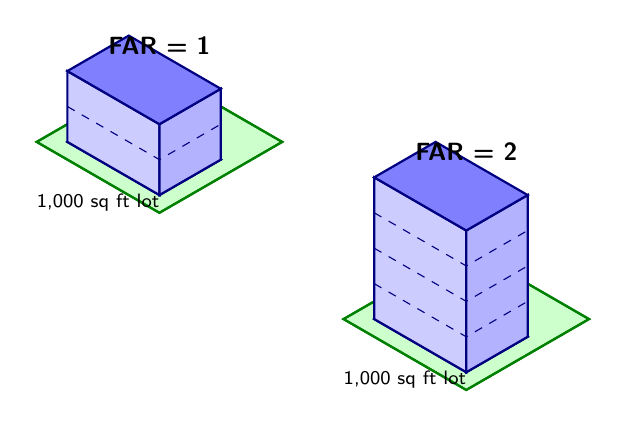
\begin{tikzpicture}[
            scale=0.45,
            x={(0.866cm,-0.5cm)},
            y={(0.866cm,0.5cm)},
            z={(0cm,1cm)},
            lot/.style={fill=green!20, draw=green!50!black, thick},
            building/.style={fill=blue!30, draw=blue!50!black, thick},
            building top/.style={fill=blue!50, draw=blue!50!black, thick},
            building side/.style={fill=blue!20, draw=blue!50!black, thick},
        ]
        % LEFT: FAR = 1
        \begin{scope}[shift={(-5,0,0)}]
            \fill[lot] (0,0,0) -- (4,0,0) -- (4,4,0) -- (0,4,0) -- cycle;
            \draw[green!50!black, thick] (0,0,0) -- (4,0,0) -- (4,4,0) -- (0,4,0) -- cycle;
            \def\bx{0.5} \def\by{0.5} \def\bw{3} \def\bd{2} \def\bh{2}
            \fill[building] (\bx,\by,0) -- (\bx+\bw,\by,0) -- (\bx+\bw,\by+\bd,0) -- (\bx,\by+\bd,0) -- cycle;
            \fill[building side] (\bx,\by,0) -- (\bx+\bw,\by,0) -- (\bx+\bw,\by,\bh) -- (\bx,\by,\bh) -- cycle;
            \fill[building] (\bx+\bw,\by,0) -- (\bx+\bw,\by+\bd,0) -- (\bx+\bw,\by+\bd,\bh) -- (\bx+\bw,\by,\bh) -- cycle;
            \fill[building top] (\bx,\by,\bh) -- (\bx+\bw,\by,\bh) -- (\bx+\bw,\by+\bd,\bh) -- (\bx,\by+\bd,\bh) -- cycle;
            \draw[blue!50!black, dashed] (\bx,\by,1) -- (\bx+\bw,\by,1) -- (\bx+\bw,\by+\bd,1);
            \node[font=\scriptsize\sffamily, below] at (2,0,-0.2) {1,000 sq ft lot};
            \node[font=\small\sffamily\bfseries, above] at (2,2,\bh+0.2) {FAR = 1};
        \end{scope}
        % RIGHT: FAR = 2
        \begin{scope}[shift={(5,0,0)}]
            \fill[lot] (0,0,0) -- (4,0,0) -- (4,4,0) -- (0,4,0) -- cycle;
            \draw[green!50!black, thick] (0,0,0) -- (4,0,0) -- (4,4,0) -- (0,4,0) -- cycle;
            \def\bx{0.5} \def\by{0.5} \def\bw{3} \def\bd{2} \def\bh{4}
            \fill[building] (\bx,\by,0) -- (\bx+\bw,\by,0) -- (\bx+\bw,\by+\bd,0) -- (\bx,\by+\bd,0) -- cycle;
            \fill[building side] (\bx,\by,0) -- (\bx+\bw,\by,0) -- (\bx+\bw,\by,\bh) -- (\bx,\by,\bh) -- cycle;
            \fill[building] (\bx+\bw,\by,0) -- (\bx+\bw,\by+\bd,0) -- (\bx+\bw,\by+\bd,\bh) -- (\bx+\bw,\by,\bh) -- cycle;
            \fill[building top] (\bx,\by,\bh) -- (\bx+\bw,\by,\bh) -- (\bx+\bw,\by+\bd,\bh) -- (\bx,\by+\bd,\bh) -- cycle;
            \foreach \h in {1,2,3} {
                \draw[blue!50!black, dashed] (\bx,\by,\h) -- (\bx+\bw,\by,\h) -- (\bx+\bw,\by+\bd,\h);
            }
            \node[font=\scriptsize\sffamily, below] at (2,0,-0.2) {1,000 sq ft lot};
            \node[font=\small\sffamily\bfseries, above] at (2,2,\bh+0.2) {FAR = 2};
        \end{scope}
        \end{tikzpicture}
        
        \vspace{0.5em}
        {\small $\text{FAR} = \dfrac{\text{Total Building Floor Area}}{\text{Lot Area}}$}
    \end{column}
    
    \begin{column}{0.43\textwidth}
        \small
        \textbf{FAR limits development intensity}
        
        \vspace{0.5em}
        Same lot, different allowed density:
        \begin{itemize}
            \item FAR = 1: Can build 1,000 sq ft
            \item FAR = 2: Can build 2,000 sq ft
        \end{itemize}
        
        \vspace{0.5em}
        \textbf{Chicago zoning examples:}
        \vspace{-0.3em}
        \begin{center}
        \scriptsize
        \begin{tabular}{lcc}
        \toprule
        Zone & Max FAR & Typical Use \\
        \midrule
        RS-3 & 0.9 & Single-family \\
        RT-4 & 1.2 & Two-flat \\
        RM-5 & 2.0 & Small apartment \\
        RM-6 & 4.4 & Mid-rise \\
        \bottomrule
        \end{tabular}
        \end{center}
    \end{column}
    \end{columns}
\end{frame}


% ==============================================================================
% SLIDE 13: WHAT IS DUPAC?
% ==============================================================================
\begin{frame}
    \frametitle{Density Outcomes: Dwelling Units Per Acre (DUPAC)}
    
    \begin{columns}[T]
    \begin{column}{0.55\textwidth}
        \centering
        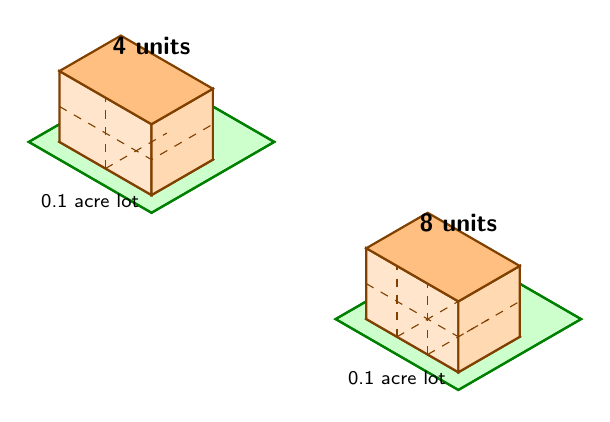
\begin{tikzpicture}[
            scale=0.45,
            x={(0.866cm,-0.5cm)},
            y={(0.866cm,0.5cm)},
            z={(0cm,1cm)},
            lot/.style={fill=green!20, draw=green!50!black, thick},
            building/.style={fill=orange!30, draw=orange!50!black, thick},
            building top/.style={fill=orange!50, draw=orange!50!black, thick},
            building side/.style={fill=orange!20, draw=orange!50!black, thick},
            unit/.style={fill=red!40, draw=red!60!black, thick},
        ]
        % LEFT: 4 units
        \begin{scope}[shift={(-5,0,0)}]
            \fill[lot] (0,0,0) -- (4,0,0) -- (4,4,0) -- (0,4,0) -- cycle;
            \draw[green!50!black, thick] (0,0,0) -- (4,0,0) -- (4,4,0) -- (0,4,0) -- cycle;
            \def\bx{0.5} \def\by{0.5} \def\bw{3} \def\bd{2} \def\bh{2}
            \fill[building] (\bx,\by,0) -- (\bx+\bw,\by,0) -- (\bx+\bw,\by+\bd,0) -- (\bx,\by+\bd,0) -- cycle;
            \fill[building side] (\bx,\by,0) -- (\bx+\bw,\by,0) -- (\bx+\bw,\by,\bh) -- (\bx,\by,\bh) -- cycle;
            \fill[building] (\bx+\bw,\by,0) -- (\bx+\bw,\by+\bd,0) -- (\bx+\bw,\by+\bd,\bh) -- (\bx+\bw,\by,\bh) -- cycle;
            \fill[building top] (\bx,\by,\bh) -- (\bx+\bw,\by,\bh) -- (\bx+\bw,\by+\bd,\bh) -- (\bx,\by+\bd,\bh) -- cycle;
            % Unit dividers
            \draw[orange!50!black, dashed] (\bx,\by,1) -- (\bx+\bw,\by,1) -- (\bx+\bw,\by+\bd,1);
            \draw[orange!50!black, dashed] (\bx+1.5,\by,0) -- (\bx+1.5,\by,\bh);
            \draw[orange!50!black, dashed] (\bx+1.5,\by,0) -- (\bx+1.5,\by+\bd,0);
            \node[font=\scriptsize\sffamily, below] at (2,0,-0.2) {0.1 acre lot};
            \node[font=\small\sffamily\bfseries, above] at (2,2,\bh+0.2) {4 units};
        \end{scope}
        % RIGHT: 8 units (same FAR, more units)
        \begin{scope}[shift={(5,0,0)}]
            \fill[lot] (0,0,0) -- (4,0,0) -- (4,4,0) -- (0,4,0) -- cycle;
            \draw[green!50!black, thick] (0,0,0) -- (4,0,0) -- (4,4,0) -- (0,4,0) -- cycle;
            \def\bx{0.5} \def\by{0.5} \def\bw{3} \def\bd{2} \def\bh{2}
            \fill[building] (\bx,\by,0) -- (\bx+\bw,\by,0) -- (\bx+\bw,\by+\bd,0) -- (\bx,\by+\bd,0) -- cycle;
            \fill[building side] (\bx,\by,0) -- (\bx+\bw,\by,0) -- (\bx+\bw,\by,\bh) -- (\bx,\by,\bh) -- cycle;
            \fill[building] (\bx+\bw,\by,0) -- (\bx+\bw,\by+\bd,0) -- (\bx+\bw,\by+\bd,\bh) -- (\bx+\bw,\by,\bh) -- cycle;
            \fill[building top] (\bx,\by,\bh) -- (\bx+\bw,\by,\bh) -- (\bx+\bw,\by+\bd,\bh) -- (\bx,\by+\bd,\bh) -- cycle;
            % More unit dividers (8 units)
            \draw[orange!50!black, dashed] (\bx,\by,1) -- (\bx+\bw,\by,1) -- (\bx+\bw,\by+\bd,1);
            \draw[orange!50!black, dashed] (\bx+1,\by,0) -- (\bx+1,\by,\bh);
            \draw[orange!50!black, dashed] (\bx+2,\by,0) -- (\bx+2,\by,\bh);
            \draw[orange!50!black, dashed] (\bx+1,\by,0) -- (\bx+1,\by+\bd,0);
            \draw[orange!50!black, dashed] (\bx+2,\by,0) -- (\bx+2,\by+\bd,0);
            \node[font=\scriptsize\sffamily, below] at (2,0,-0.2) {0.1 acre lot};
            \node[font=\small\sffamily\bfseries, above] at (2,2,\bh+0.2) {8 units};
        \end{scope}
        \end{tikzpicture}
        
        \vspace{0.5em}
        {\small DUPAC: 40 vs.\ 80 units/acre  (same building volume!)}
    \end{column}
    
    \begin{column}{0.43\textwidth}
        \small
        \textbf{DUPAC captures population density}
        
        \vspace{0.5em}
        $\text{DUPAC} = \dfrac{\text{\# Dwelling Units}}{\text{Lot Acreage}}$
        
        \vspace{0.5em}
        \textbf{Why both measures?}
        \begin{itemize}
            \item Same FAR, different DUPAC
            \item \textbf{Developers} care about FAR (total rentable space)
            \item \textbf{Neighbors} care about DUPAC (congestion, parking, schools)
        \end{itemize}
    \end{column}
    \end{columns}
\end{frame}


% ==============================================================================
% SLIDE 14: DATA - NEW MULTIFAMILY CONSTRUCTION
% ==============================================================================
\begin{frame}
    \frametitle{Data: New Multifamily Construction}
    
    \begin{columns}[T]
    \begin{column}{0.55\textwidth}
    \textbf{Source}: Cook County Assessor parcel data, 2006-2025
    
    \vspace{0.5em}
    \textbf{Sample}: Multifamily buildings with 2--100 units
    \begin{itemize}
        \item \textbf{Single family}: Majority of construction but less variation in density
        \item \textbf{Large developments} (100+ units): Planned Development process with more city oversight
    \end{itemize}
    
    \vspace{0.5em}
    \textbf{Why multifamily matters}: 
    \begin{itemize}
        \item Only $\sim$19\% of new construction but a dispraportionate share of total housing supply
    \end{itemize}
    \end{column}
    
    \begin{column}{0.43\textwidth}
    \textbf{Summary statistics}:
    \vspace{0.3em}
    \small
    \begin{tabular}{lcc}
    \toprule
     & All & MF Only \\
    \midrule
    Avg FAR & 1.22 & 2.32 \\
    Avg Units & 6.65 & 31.3 \\
    Avg Stories & 2.27 & 2.75 \\
    Avg DUPAC & 28.5 & 74.5 \\
    \midrule
    N & 13,236 & 2,469 \\
    \bottomrule
    \end{tabular}
    \end{column}
    \end{columns}
\end{frame}


% ==============================================================================
% SLIDE 15: IDENTIFICATION STRATEGY
% ==============================================================================
\begin{frame}
    \frametitle{Identification Strategy: Border Discontinuity}
    
    \textbf{Idea}: Compare new multifamily construction on opposite sides of ward boundaries
    \begin{itemize}
        \item Focus on parcels \textbf{within 500 feet} of border 
        \item Use stringent border-pair $\times$ year FEs to remove unobserved heterogeneity
    \end{itemize}
    
    \vspace{0.3em}
    \textbf{Identifying variation}: At the same border in the same year, does the stricter side have less dense construction?
    
    \vspace{0.3em}
    Two specifications:
    \begin{itemize}
        \item \textbf{Visual RD}: Descriptive, visual evidence of discontinuities at ward borders
        \item \textbf{Regressions}: Regression with continuous strictness measure and stringent FEs
    \end{itemize}
\end{frame}


% ==============================================================================
% SLIDE 16: VISUAL RD RESULTS
% ==============================================================================
\begin{frame}[label=visual-rd-main]
    \frametitle{Visual Evidence: Density Discontinuity at Ward Borders}
    
    \begin{columns}[T]
    \begin{column}{0.48\textwidth}
        \centering
        \textbf{Log(FAR)}
        \begin{figure}
            \includegraphics[width=\textwidth,height=0.55\textheight,keepaspectratio]{../tasks/spatial_rd_same_zone_only/output/rd_plot_log_density_far_bw500_triangular.pdf}
        \end{figure}
    \end{column}
    \begin{column}{0.48\textwidth}
        \centering
        \textbf{Log(DUPAC)}
        \begin{figure}
            \includegraphics[width=\textwidth,height=0.55\textheight,keepaspectratio]{../tasks/spatial_rd_same_zone_only/output/rd_plot_log_density_dupac_bw500_triangular.pdf}
        \end{figure}
    \end{column}
    \end{columns}
    
    \scriptsize
    \textit{Notes}: Stacked borders; lenient (left) vs.\ strict (right). 500 ft bandwidth.
    
    \vfill\hfill
    \hyperlink{visual-rd-placebo}{\beamergotobutton{Placebo Boundaries}}
    \hspace{0.2em}
    \hyperlink{visual-rd-functional}{\beamergotobutton{Functional Form}}
    \hspace{0.2em}
    \hyperlink{visual-rd-donut}{\beamergotobutton{Donut}}
\end{frame}


% ==============================================================================
% SLIDE 17: BORDER-PAIR FE RESULTS
% ==============================================================================
\begin{frame}[label=density-reg-main]
    \frametitle{Main Results: Border-Pair Fixed Effects}
    
    \small
    \textbf{Specification}: 
    $\ln(Y_i) = \beta \cdot \text{Strictness}_i + \alpha_{\text{border} \times \text{year} } + \varepsilon_i$\\
    Sample: Within 500 ft, 2-100 units. Standard errors clustered at border-pair level.
    
    \begin{center}
    \input{../tasks/border_pair_FE_regressions/output/fe_table_bw500_pair_x_year.tex}
    \end{center}
    
    \vspace{0.1em}
    \textbf{Interpretation}: A 1 SD $\uparrow$ in strictness $\rightarrow$ 13-15\% less dense multifamily construction
    
    \vspace{-0.4em}
    \vfill\hfill
    \hyperlink{density-reg-bw250}{\beamergotobutton{250ft}}
    \hspace{0.1em}
    \hyperlink{density-reg-bw1000}{\beamergotobutton{1000ft}}

\end{frame}
